% fig01_pipeline.tex — TikZ 7-stage antimatter-factory flow diagram for §Full Pipeline.
% Compiled by the paper Makefile via `make figures` (pdflatex on the snippet).
% Tier-color-coded: green = closed-form / numerical PASS (closed in this funnel),
% orange = wet-lab / measured-oracle boundary (NOT closed). The tier word is inside
% the node so the diagram is independently readable without the §Full Pipeline table.
%
% Manual single-shot compile (debug):
%   pdflatex -interaction=nonstopmode -halt-on-error fig01_pipeline.tex
\documentclass[tikz,border=4pt]{standalone}
\usetikzlibrary{positioning,arrows.meta,shapes.geometric}
\begin{document}
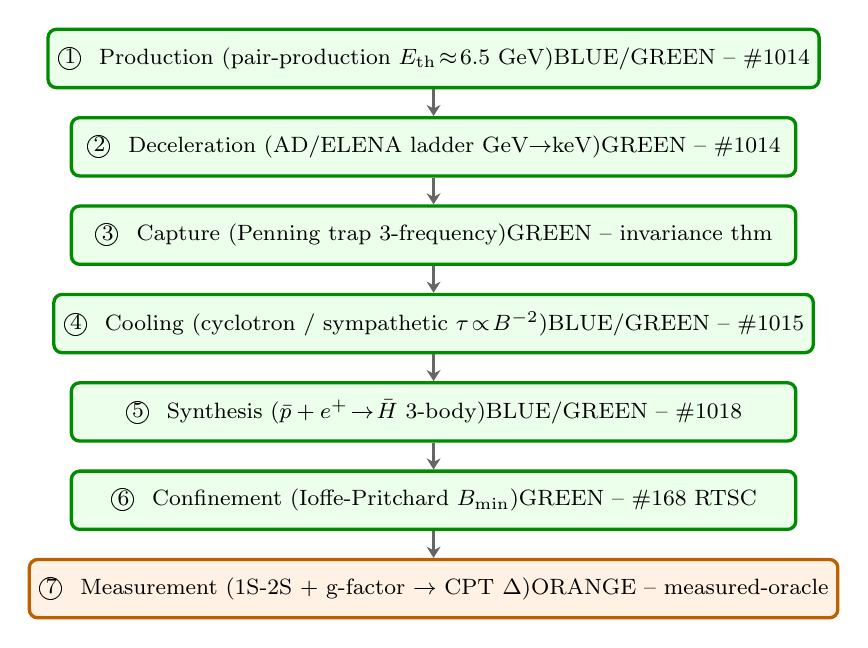
\begin{tikzpicture}[
  font=\footnotesize,
  closed/.style = {
    rectangle, rounded corners=3pt, draw=green!55!black, very thick,
    minimum width=9.2cm, minimum height=0.74cm, align=left,
    fill=green!8,
  },
  wet/.style = {
    rectangle, rounded corners=3pt, draw=orange!75!black, very thick,
    minimum width=9.2cm, minimum height=0.74cm, align=left,
    fill=orange!10,
  },
  arrow/.style = {-{Stealth[length=4pt,width=5pt]}, thick, draw=black!60},
  node distance=0.34cm,
]
  \node[closed]               (s1) {\textcircled{1}\ \ Production (pair-production $E_{\mathrm{th}}\!\approx\!6.5$ GeV)\hfill BLUE/GREEN -- \#1014};
  \node[closed, below=of s1]  (s2) {\textcircled{2}\ \ Deceleration (AD/ELENA ladder GeV$\to$keV)\hfill GREEN -- \#1014};
  \node[closed, below=of s2]  (s3) {\textcircled{3}\ \ Capture (Penning trap 3-frequency)\hfill GREEN -- invariance thm};
  \node[closed, below=of s3]  (s4) {\textcircled{4}\ \ Cooling (cyclotron / sympathetic $\tau\!\propto\!B^{-2}$)\hfill BLUE/GREEN -- \#1015};
  \node[closed, below=of s4]  (s5) {\textcircled{5}\ \ Synthesis ($\bar p+e^+\!\to\!\bar H$ 3-body)\hfill BLUE/GREEN -- \#1018};
  \node[closed, below=of s5]  (s6) {\textcircled{6}\ \ Confinement (Ioffe-Pritchard $B_{\min}$)\hfill GREEN -- \#168 RTSC};
  \node[wet,    below=of s6]  (s7) {\textcircled{7}\ \ Measurement (1S-2S + g-factor $\to$ CPT $\Delta$)\hfill ORANGE -- measured-oracle};

  \draw[arrow] (s1) -- (s2);
  \draw[arrow] (s2) -- (s3);
  \draw[arrow] (s3) -- (s4);
  \draw[arrow] (s4) -- (s5);
  \draw[arrow] (s5) -- (s6);
  \draw[arrow] (s6) -- (s7);
\end{tikzpicture}
\end{document}
